\documentclass{article}
\usepackage[utf8]{inputenc}

\title{CMSC6950 PROJECT}
\author{Jingyao li }
\date{June 2021}

\newpage

\usepackage{natbib}
\usepackage{graphicx}

\begin{document}

\maketitle

\section{Introduction}
This task was intended to allow me to visualize data in Python. I use the Conda environment and the various packages that are required. Stored communication and presentation through the use of git hub.
Gala is a Python pack associated with astropy, designed to provide an efficient tool for performing common tasks in galactic dynamics studies. Most of this code uses Python for flexible, friendly interfaces that interact with wrappers in the underlying code (primarily C) for fast calculations. Common operations include gravitational potential and force assessment, orbital integration, dynamic coordinate transformation, and chaos indicators for calculating nonlinear dynamics. Gala turns heavily on the units and astroastropy coordinate system defined in the core pack (Astropy). Units and astrophic yes. coordinates).
In this project, I demonstrated my ability to use Python through Gala: A Python package for galactic dynamics.



\maketitle
\section

\newpage
\section{Results}
 There are two checkpoint in the project. And the result shows in the img file.
 These are figures for checkpoint1.
\includegraphics[scale=0.6]{fpotential.integrate_orbit.png}
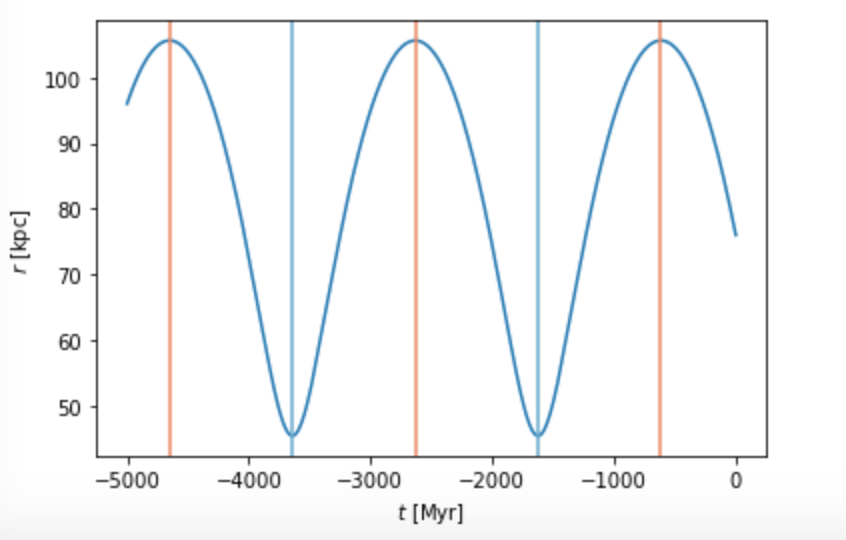
\includegraphics[scale=0.6]{spherical.png}
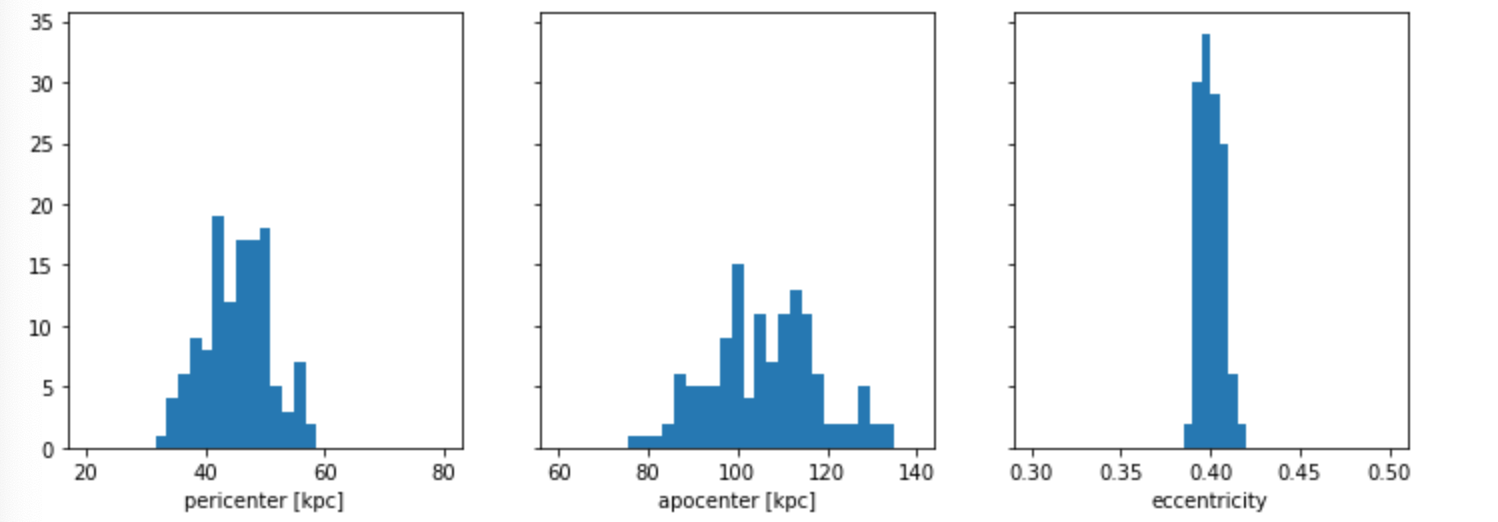
\includegraphics[scale=0.6]{pericenter_apocenter_eccentricity.png}
 These are figures for checkpoint2.
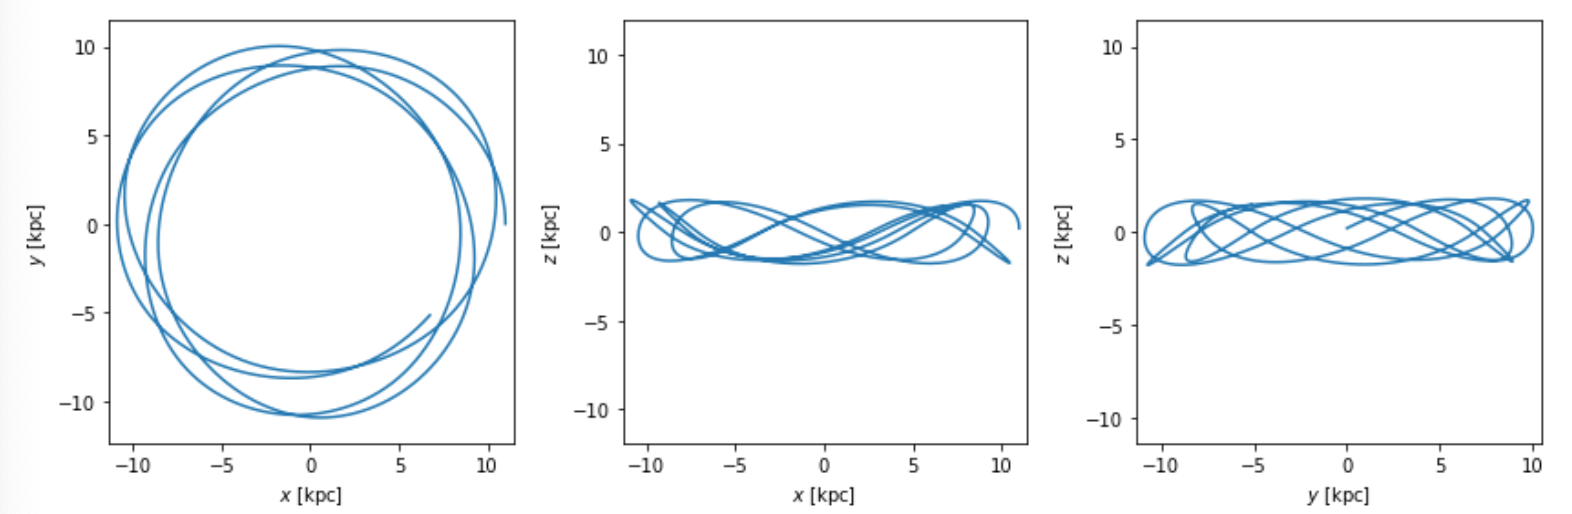
\includegraphics[scale=0.6]{integrate_orbit.png}
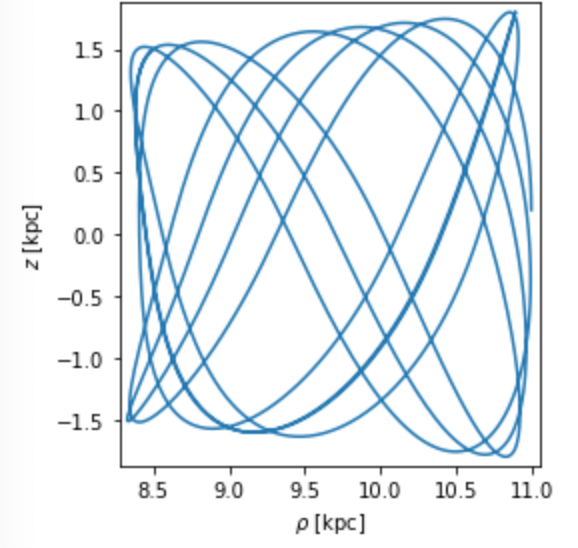
\includegraphics[scale=0.6]{cylindrical.png}



\newpage
\section{Conclusion}
Python has mighty expressive power. In terms of visualization of graphics, it can express information effectively in real-time according to data. Git hub also plays a beneficial role. In this experiment, the main data are transmitted through Git. Another good thing to say about Conda is that it's so easy to download and add packages.
\citep{}
\section{contributors}
Main author: Adrian Price-Whelan (@adrn)
Johnny Greco
Sergey Koposov
Daniel Lenz
Pey Lian Lim
Syrtis Major
Semyeong Oh
Brigitta Sipocz
Nathaniel Starkman
\bibliographystyle{plain}
\bibliography{references}
\end{document}
